\label{chap:impl}

 \subsection{Hardware Details}

\begin{figure}[hb] \centering
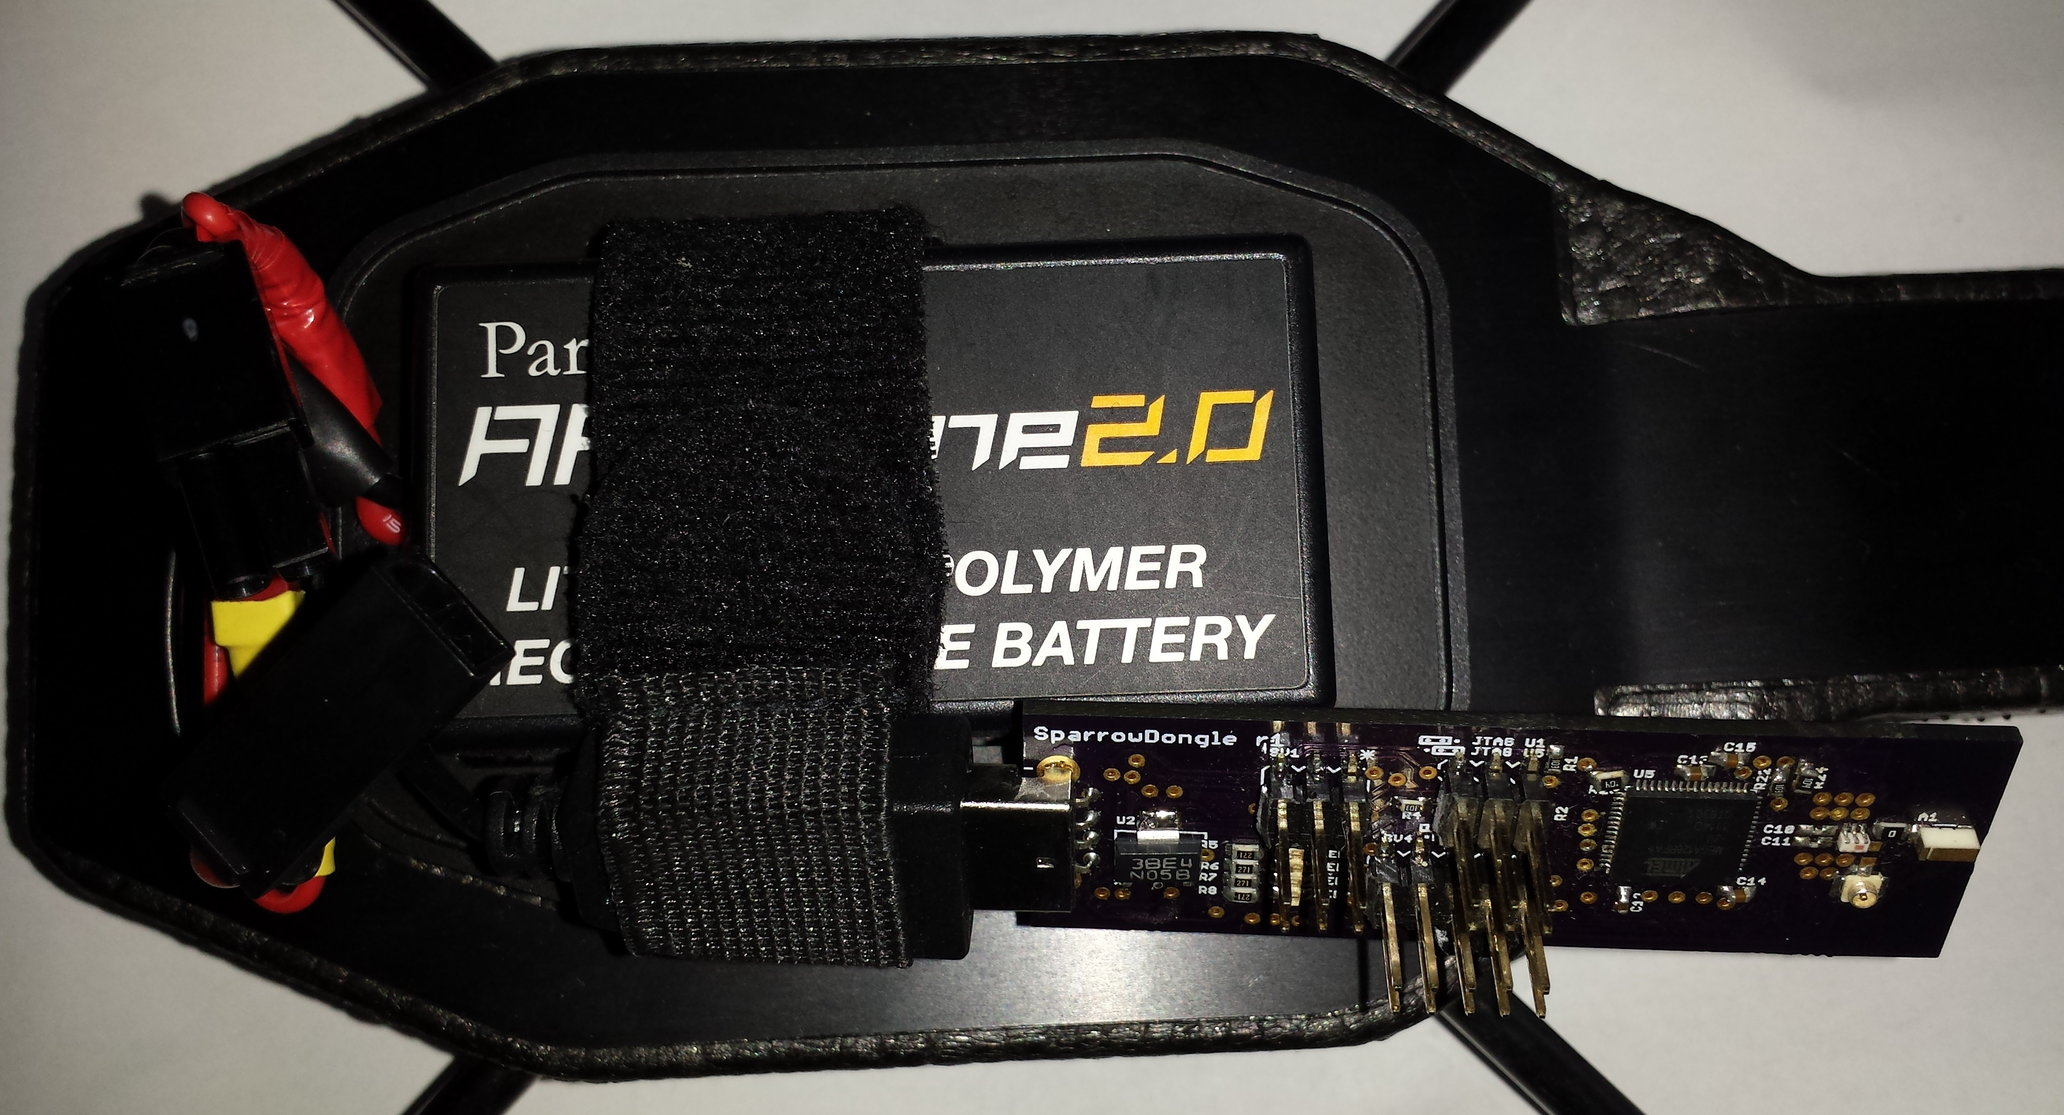
\includegraphics[width=0.45\textwidth]{img/dronedongle.jpg} \caption{SparrowDongle connected to AR Parrot Drone 2.0 } \end{figure}

The hardware components used are the following:
\begin{itemize}

\item a SparrowDongle with two micro controllers: The 8-bit ATMega128RFA1 which has an on-chip 2.4GHz wireless transceiver and the ATMega32U4, both from Atmel.

\item a SparrowV3.2  with an ATMega128RFA1 micro controller 

\item a AR Parrot Drone v2.0

\item a SAMSUNG Galaxy S4 with android 4.4.2, but a laptop or other mobile phones with android/ios can be used for controlling the drone

\end{itemize}

Because of the addition of the SparrowDongle, the drone's polyester hull has had to been carved a little in order to accommodate it.
 

\subsection{Software Implementation}

The parrot drone, with a Linux based operating system, allow the software to be organized in different modules. The modules can be modified individually  to add more features to the system.

The SparrowDongle gateway dumps every data received on the serial. It is always in a listen for data state. When it receives the data, it sends back an ack to let the SparrowV3.2 node know that it can begin sending the entire data to the mobile gateway. 

The SparrowV3.2 node is sending periodically a small data packet to check if a gateway is available. When it receives the ack for the packet it starts sending the stored data to the gateway. The data sent can vary, from sensor readings, to debugging informations in order to check the state of the Wireless Sensor Network.

The data gathered by the gateway is saved into different files the AR Parrot Drone's internal memory. The file also contains informations about the node identification tag and time of the transfer. The data can be accessed at any time by any device connected to the drone's wireless network via FTP.



All the collected data is processed on the drone. It awaits a socket connection in order to start sending informations regarding the state of the connected nodes.

The nodes can be programmed to determine the signal strength of the surrounding nodes. This data is sent to the drone in order to determine the approximate location of the nodes\cite{savarese2001location}.

